% (C) Marc Lijour, 2018 
% Licensed under a Creative Commons License BY-SA
% https://creativecommons.org/licenses/by-sa/2.5/ca/
% Presentation for FEA Consulting
%       Toronto: Jan 30, 2018 at 9 am
%	ConsenSys Office
% authored by Marc Lijour, January 2018
% 
% ======================================================================================================
%                                     Digital Infrastructure and Freedom
% ======================================================================================================
\section{Freedom Blossoms}

\begin{frame}
	\frametitle{Settling in the New World}
	\begin{figure} % e
		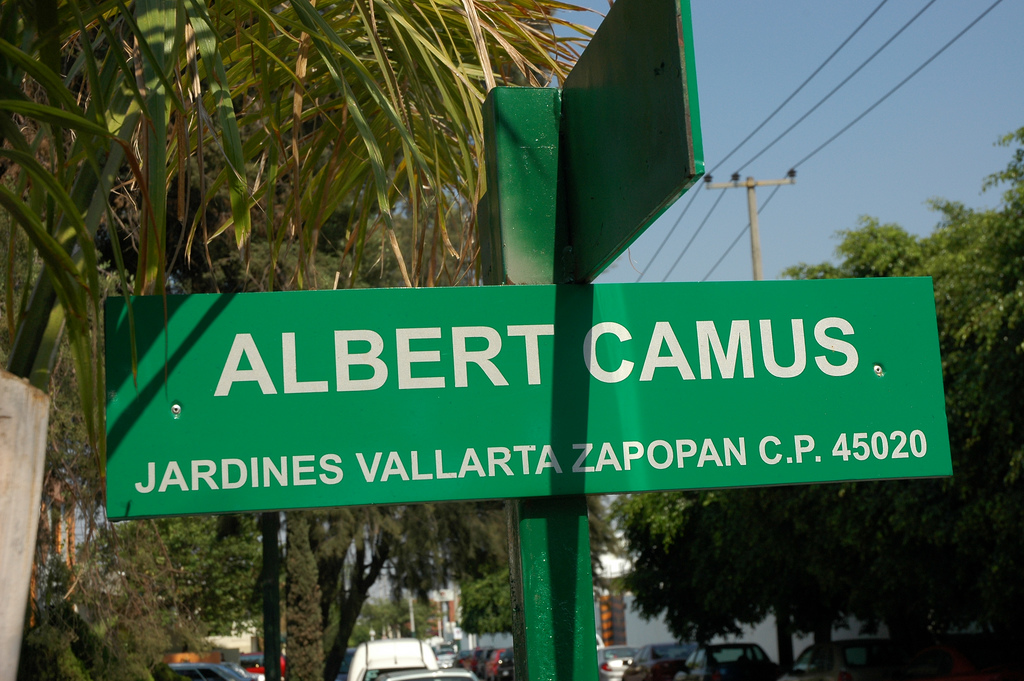
\includegraphics[width=10cm]{../pics/wonderlane2009-guadalajara_Albert_Camus}
	\end{figure}
	\tiny \copyright \href{https://www.flickr.com/photos/wonderlane/3527244519}{Wonderlane (2009)} (CC-BY license)
\end{frame}


\frame{
	\frametitle{Short History of Software}
	\framesubtitle{The birth of UNIX}
%	\framesubtitle{The birth of UNIX (Pic by Peter Hamer [\href{http://creativecommons.org/licenses/by-sa/2.0}{CC BY-SA 2.0}], via Wikimedia Commons)}
	\begin{figure}
	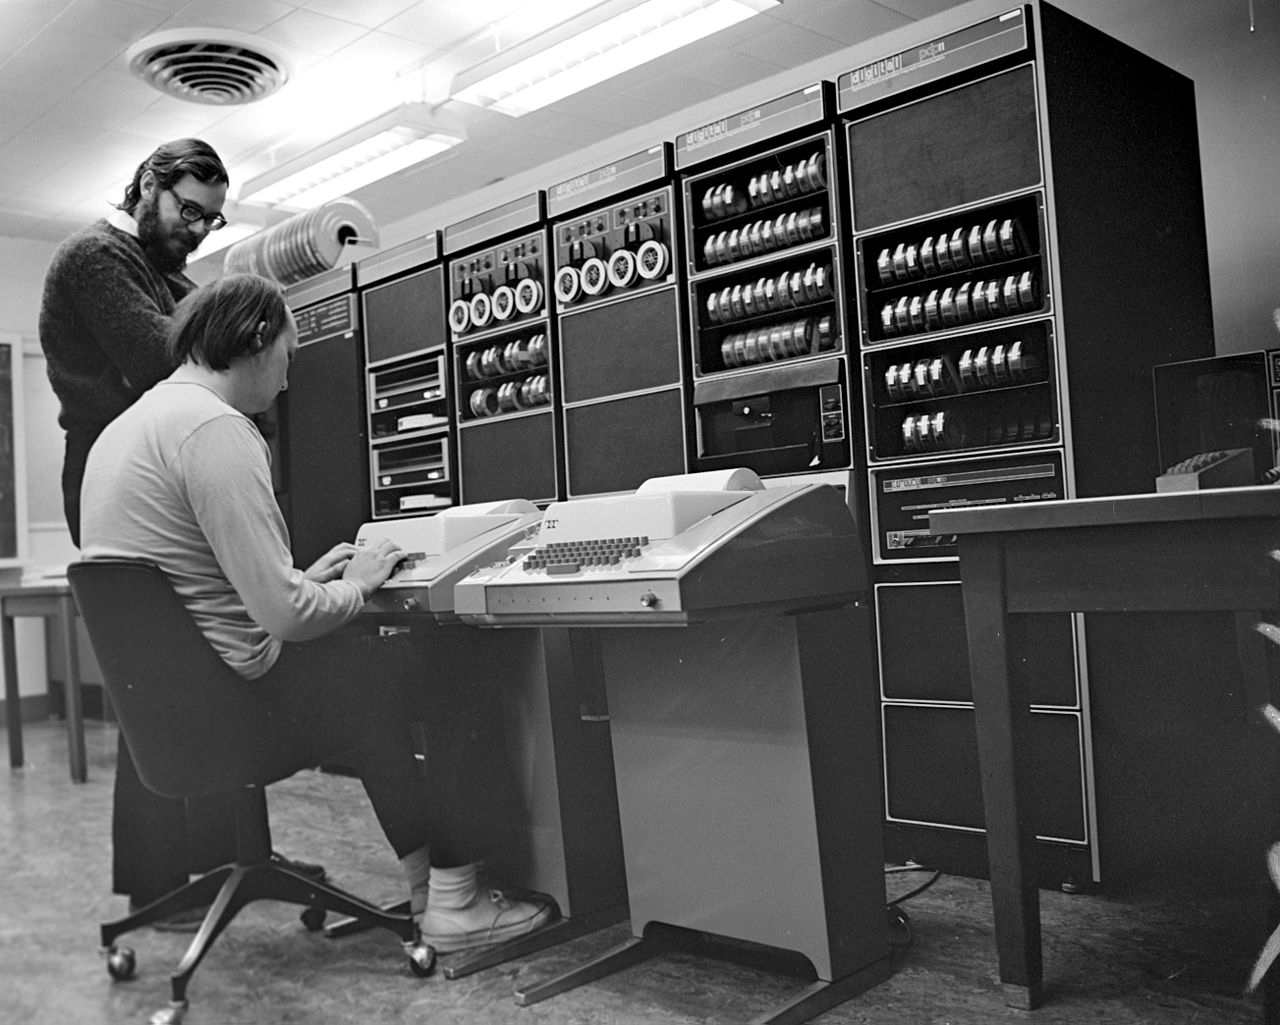
\includegraphics[height=6.4cm]{../pics/Ken_Thompson_(sitting)_and_Dennis_Ritchie_at_PDP-11_(2876612463)}
	\caption{Ken Thompson (sitting) and Dennis Ritchie at PDP-11}
	\end{figure}
	\tiny \copyright \href{http://creativecommons.org/licenses/by-sa/2.0}{Peter Hamer} (CC BY-SA 2.0 license)
}

\begin{frame}   % the four freedoms
	\frametitle{Free Software}
	\begin{figure}
		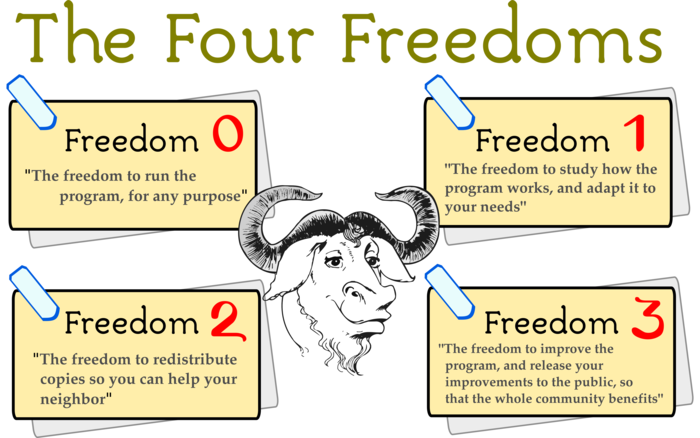
\includegraphics[width=11cm]{../pics/scaled_full_00c40105cea4c0aa3e9f}
	\end{figure}
\end{frame}

\frame{ % https://coincenter.org/entry/what-is-open-source-and-why-is-it-important-for-cryptocurrency-and-open-blockchain-projects
	\frametitle{The Cathedral \& The Bazaar (\citeyear{raymond2001})}
	\framesubtitle{A new way to develop complex bodies of software}
	\begin{columns}
	\column{0.3\textwidth}
		\begin{figure}
		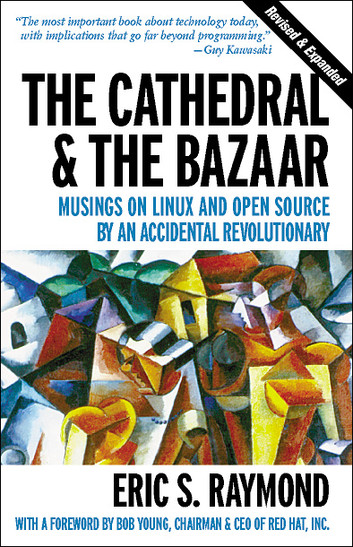
\includegraphics[width=3cm]{../pics/the-cathedral-the-bazaar}
		\end{figure}
	\column{0.7\textwidth}
	\begin{itemize}
        \item ``scratching a developer's personal itch''
        \item reuse don't rewrite
        \item pass the baton
        \item so-called \emph{Linus's Law}: ``given enough eyeballs, all bugs are shallow''
    \end{itemize}
	\end{columns}
}

\frame{
	\frametitle{Free Software and Open Source Software}
%	\framesubtitle{An introduction to Free/Libre Open Source Software (\href{https://www.youtube.com/watch?v=Tyd0FO0tko8}{Intel, 2014})}
	\framesubtitle{An introduction to Free/Libre Open Source Software (\cite{intel2014:FLOSS})}
	\begin{figure}
	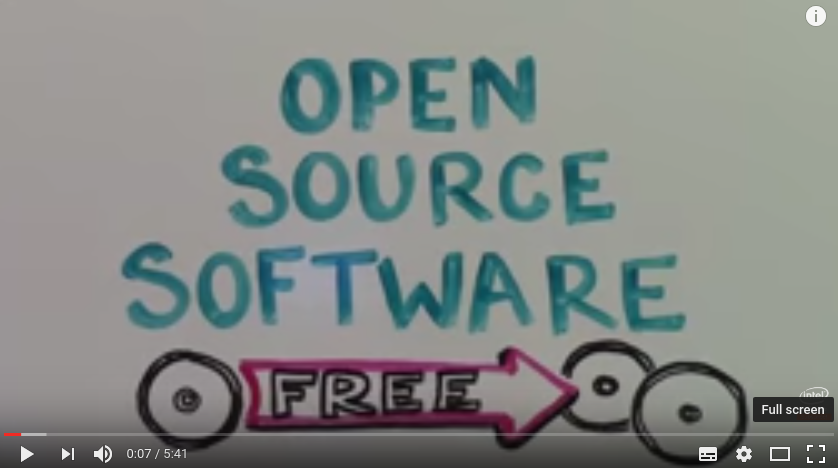
\includegraphics[height=5cm]{../pics/intel-FLOSS-intro}
	\caption{\url{https://www.youtube.com/watch?v=Tyd0FO0tko8}}
	\end{figure}
	\tiny \copyright \href{https://www.youtube.com/watch?v=Tyd0FO0tko8}{Intel Software (2014)}
}

\begin{frame}
	\frametitle{Open Source runs (almost) Everything}
	\framesubtitle{2015 was an inflexion point}
	\begin{figure} % extracts from articles and other sources published on the Web
		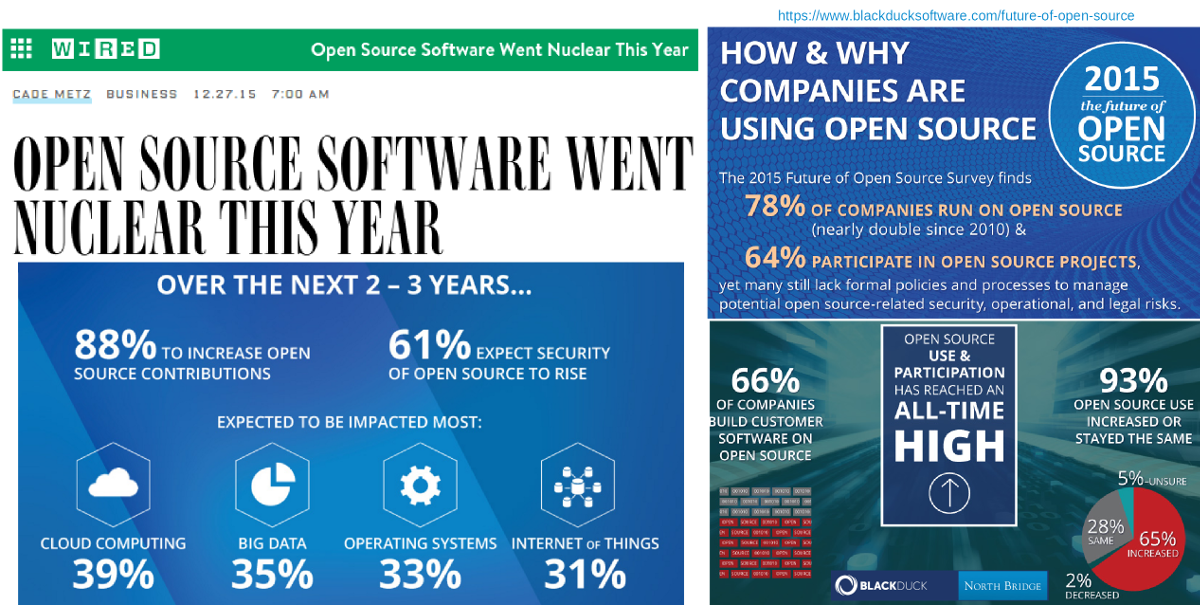
\includegraphics[width=11cm]{../pics/pic-open-source-went-nuclear-non-interlaced}
	\end{figure}
\end{frame}

\frame{
	\begin{block}{}
		\begin{quote}
			{\Huge 20\% of the world's economy will be digital by 2020.} \\
			\vspace{1em}
			\hfill ---Accenture \#techvision2016
		\end{quote}
	\end{block}
}

\frame{
	\frametitle{Blockchain is Open/Free by design}
	\framesubtitle{Starting with its first \emph{killer app}: Bitcoin}
	\begin{figure}
	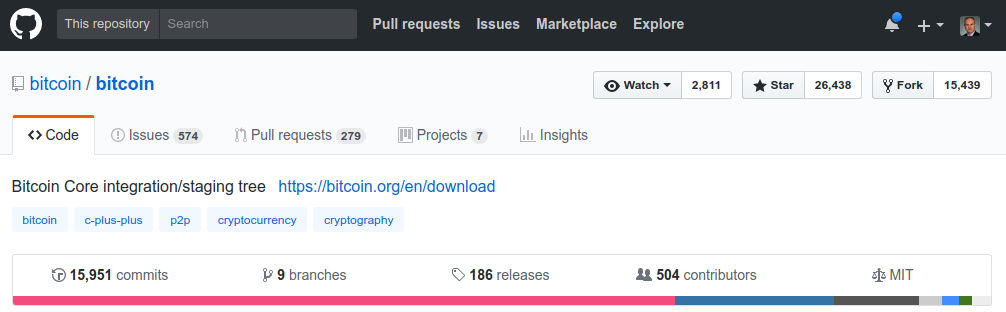
\includegraphics[width=10cm]{../../pics/bitcoin-core-github}
	\end{figure}
}

\frame{
	\frametitle{The Ethos of Blockchain is built on Openness and Decentralization}
	\begin{figure}
	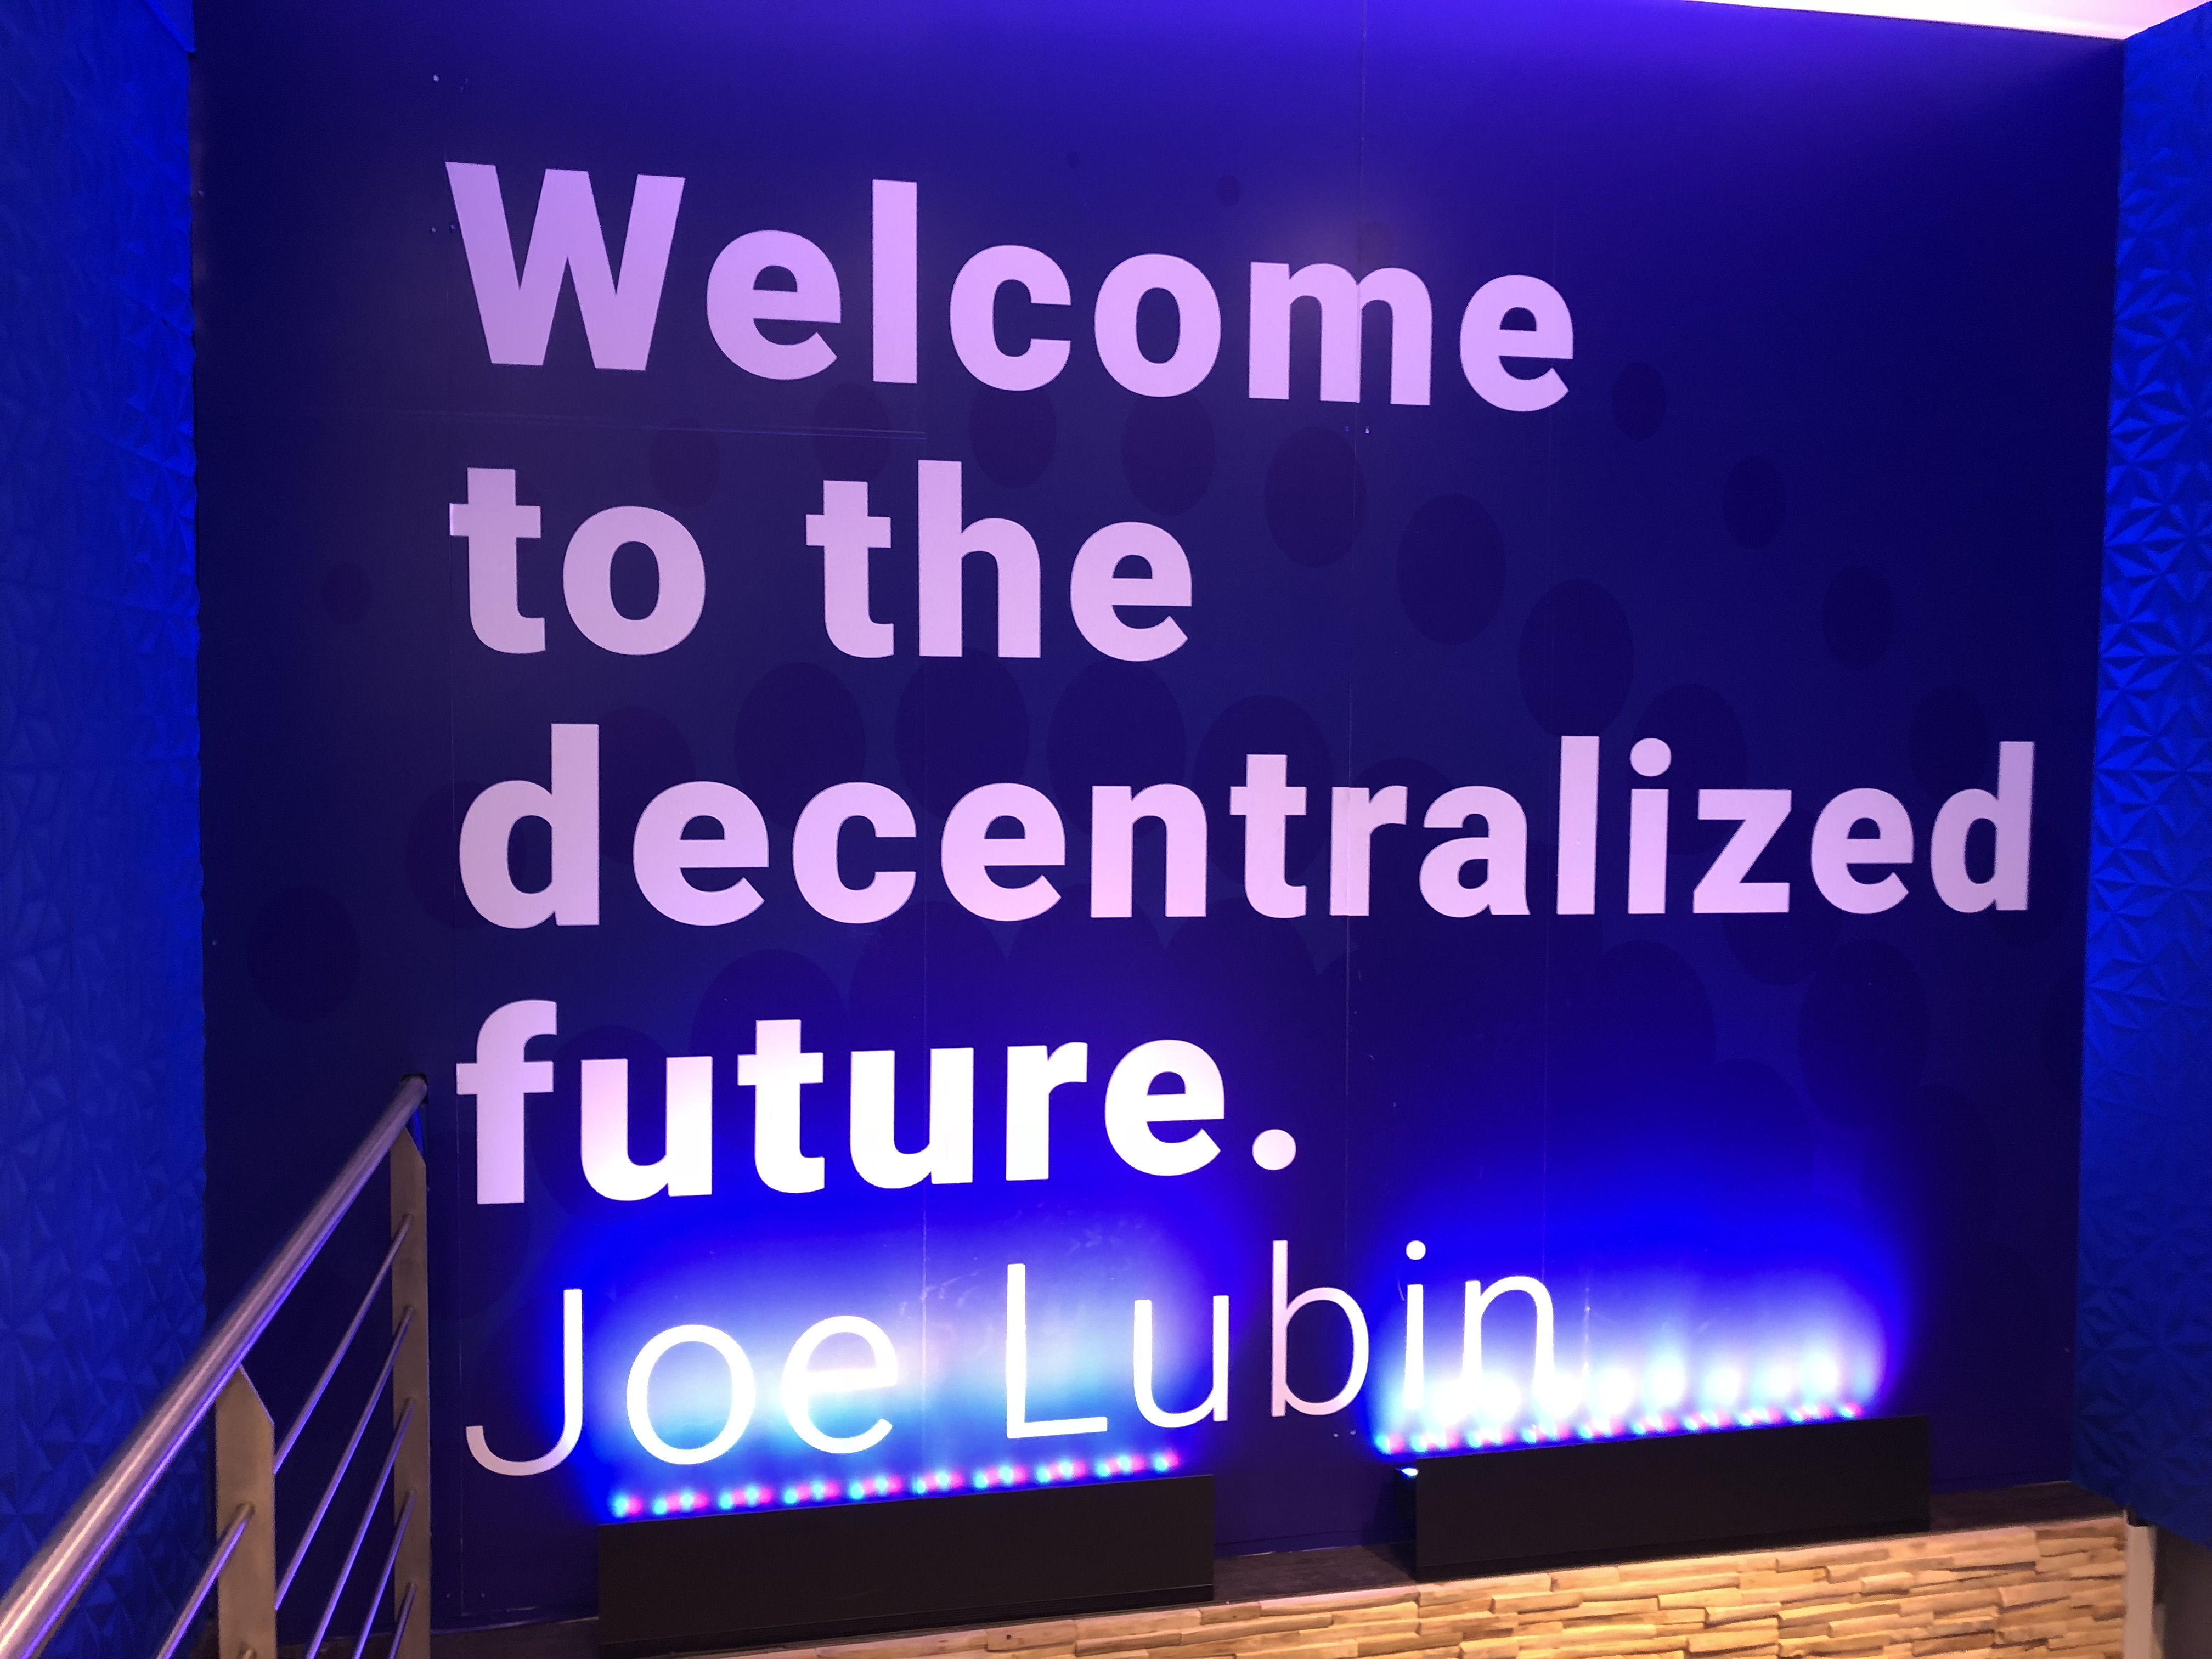
\includegraphics[width=10cm]{../../pics/ethereum/lubin_davos}
	\end{figure}
}

\frame{
	\frametitle{From IoT to Cloud and AI, and of course Blockchain}
	\begin{figure}
	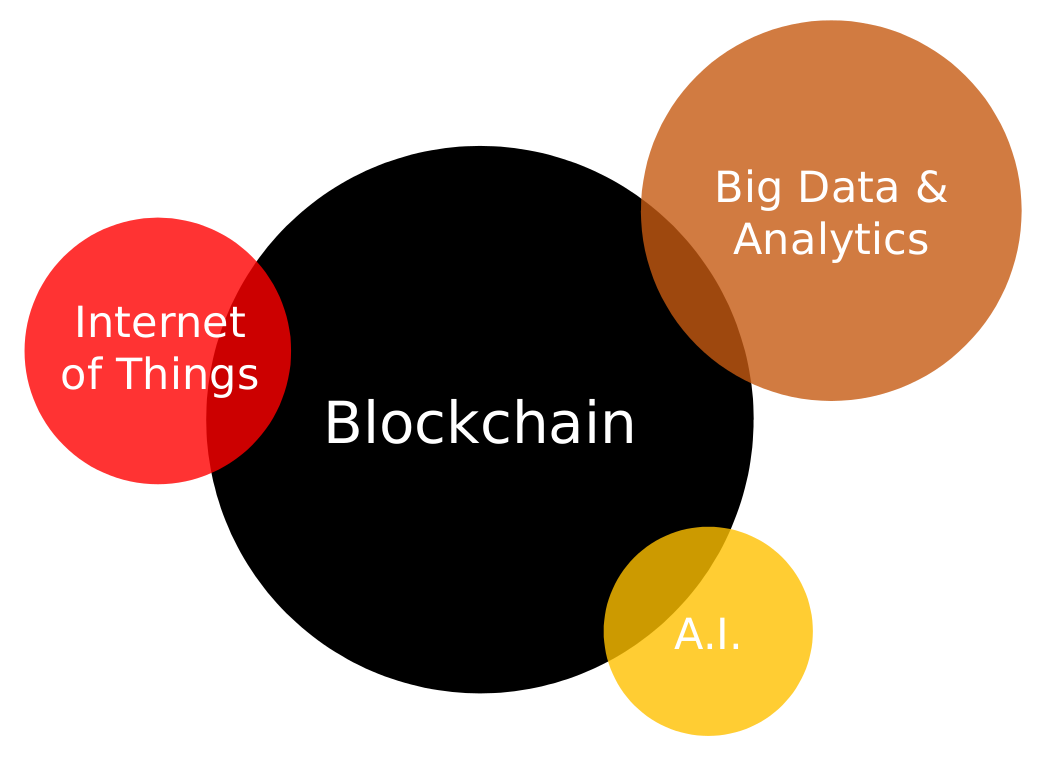
\includegraphics[width=10cm]{../../pics/colliderx/blockchain-plus-AI-etc}
	\end{figure}
}

\frame{
	\frametitle{The Milenials}
	\begin{figure} % https://www.flickr.com/photos/statefarm/26663820390
		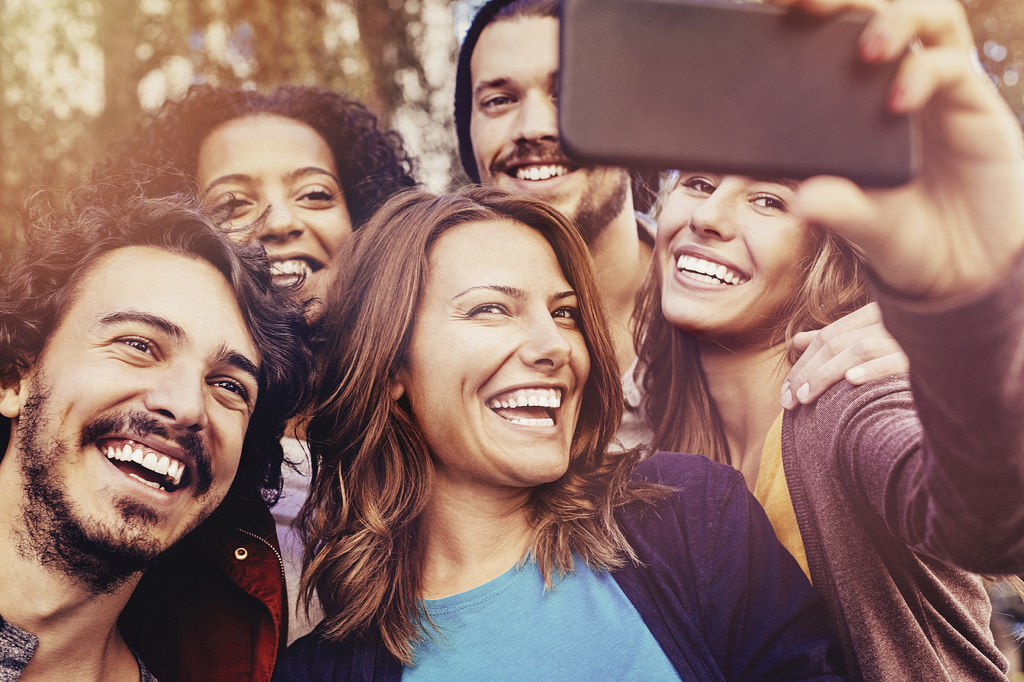
\includegraphics[width=11cm]{../pics/statefarm-milenials-CC-BY}
	\end{figure}
	\tiny \copyright \href{https://www.flickr.com/photos/statefarm/26663820390}{State Farm} (CC-BY license)
}


% ======================================================================================================
%                                     Difficulty to Fund the Commons
% ======================================================================================================
\section{The Tragedy of the Commons}

\frame{
	\frametitle{The Tragedy of the Commons}
	\begin{figure}
	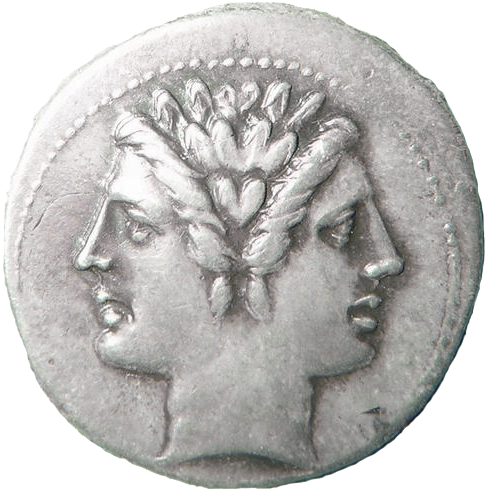
\includegraphics[width=6cm]{../pics/janus_coin}
	\end{figure}
}

\frame{
	\frametitle{Creative Chaos}
	\begin{figure} % https://www.cnbc.com/2017/11/09/just-8-percent-of-open-source-blockchain-projects-are-still-active.html
	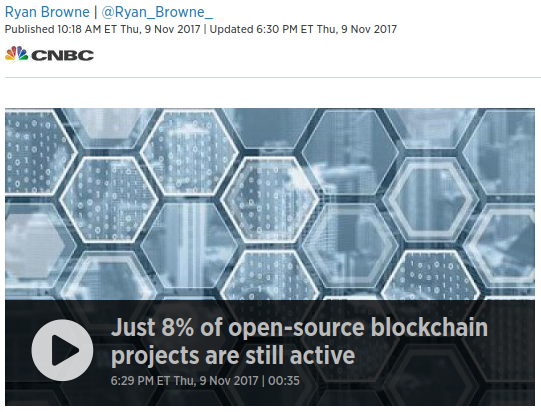
\includegraphics[width=10cm]{../pics/cnbc2017_deloitte_on_open_source_bc}
	\end{figure}
}

% Good slide -resumed in one line in the next slide
%\frame{
%	\frametitle{Starting your own Free/Libre Open Source Software project}
%	\framesubtitle{Nicely summarized by Roberto Di~Cosmo (\citeyear{dicosmo:achieving-impact})}
%	\begin{figure}
%	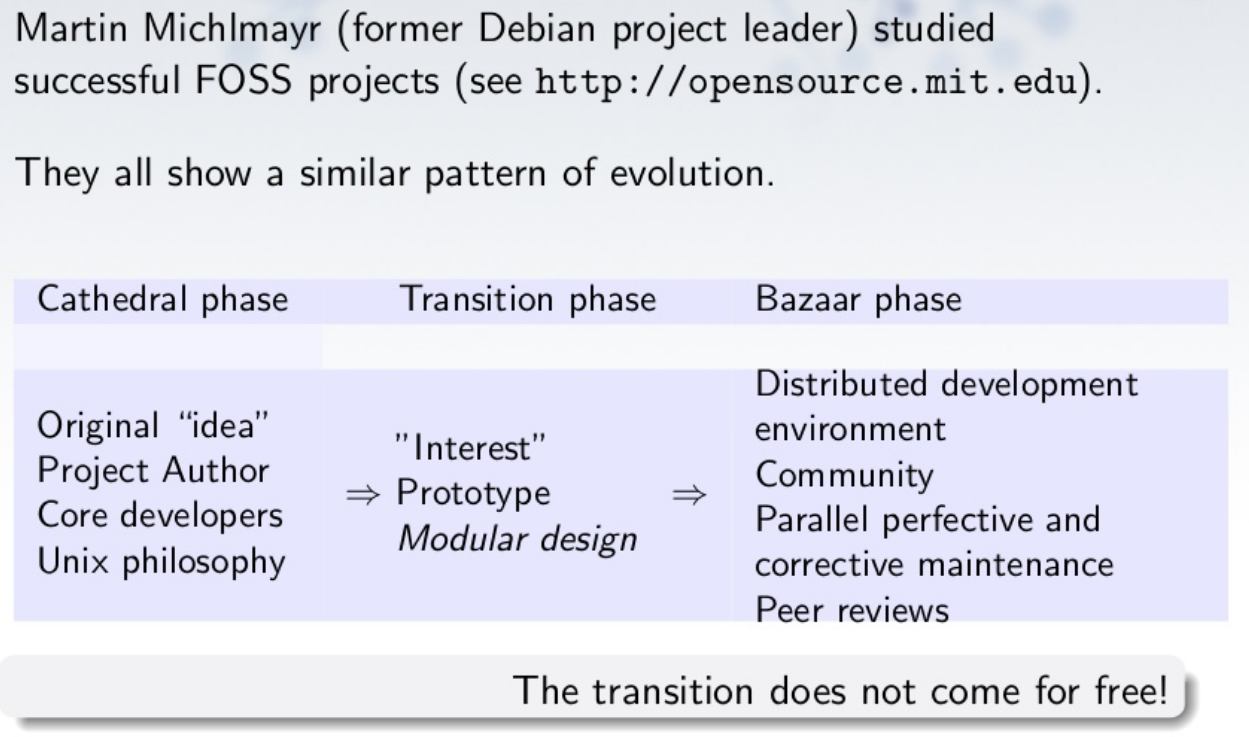
\includegraphics[width=7cm]{../../pics/dicosmo-successful-project}
%	\end{figure}
%	\begin{itemize}
%        \pause
%        \item Identify a need
%        \pause
%        \item Build a prototype
%        \pause
%        \item Grow a community
%        \pause
%        \item Set up an ecosystem \\
%                (users, developers, architects, designers, service providers...)
% the last two are the most difficult
%    \end{itemize}
%}

\frame{
	\frametitle{Nadia Eghbal's report (\citeyear{eghbal2016})}
	\framesubtitle{Roads and Bridges: The Unseen Labor Behind Our Digital Infrastructure}
	\begin{columns}
	\column{0.3\textwidth}
		\begin{figure}
		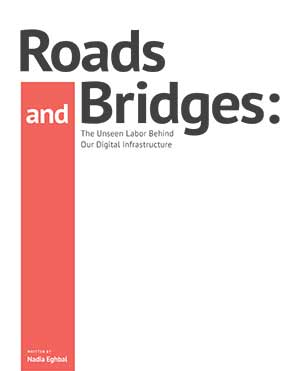
\includegraphics[width=3cm]{../pics/logos/roads-and-bridges}
		\end{figure}
	\column{0.7\textwidth}
	\begin{itemize}
        \item Open Source Software runs core infrastructure services
        \item It is poorly funded (e.g. OpenSSL)
        \item Who should fund roads and bridges?
    \end{itemize}
	\end{columns}
}

\frame{
	\frametitle{Challenges with Free/Libre Open Source Software}
	\begin{itemize}
	\item Lack of funding for the digital ``roads and bridges'' (\cite{eghbal2016}) 
        \pause
	\item Starting a Free Software project is hard, especially moving from the Cathedral phase to the Bazaar phase (\cite{dicosmo:achieving-impact})
        \pause
	\item Lack of package maintainers
        \pause
	\item Fragility and constraints of any software project (beyond open source)
	\begin{itemize}
		\item Ability (and need) to run software to open archived files
		\pause
		\item Deletion or lack of back-ups\\
			{\small \emph{(in 1999, 40\% of companies had lost or thrown away the source code of their systems)}}
		\pause
		\item Project shutdown (e.g. Google Code circa 2014)
		\pause
		\item Repository taken hostage (e.g. Code Spaces) % https://www.infoworld.com/article/2608076/data-center/murder-in-the-amazon-cloud.html
		\pause
		\item The half-life of an URL is about 4 years
	\end{itemize}
    \end{itemize}
}

\frame{
	\frametitle{The universal software archive}
    \framesubtitle{https://www.softwareheritage.org}
	\begin{figure}
	
\includegraphics[width=10cm]{../pics/software_heritage}
	\end{figure}
}

\frame{
	\frametitle{A few tips to fund Free/Libre Open Source Software}
	\framesubtitle{see also Nadia Eghbal (\citeyear{eghbal:funding})}
	\begin{itemize}
	\item Individual Time
	\pause
	\item Community support (tee-shirt sales, ads, DVD burning, donations)
	\pause
	\item Corporate investment
	\pause
	\item Sales (licensing)
	\pause
	\item Large Donations and Grants
	\end{itemize}
}

\frame{
	\frametitle{Bounties Network}
	\begin{figure} % 
		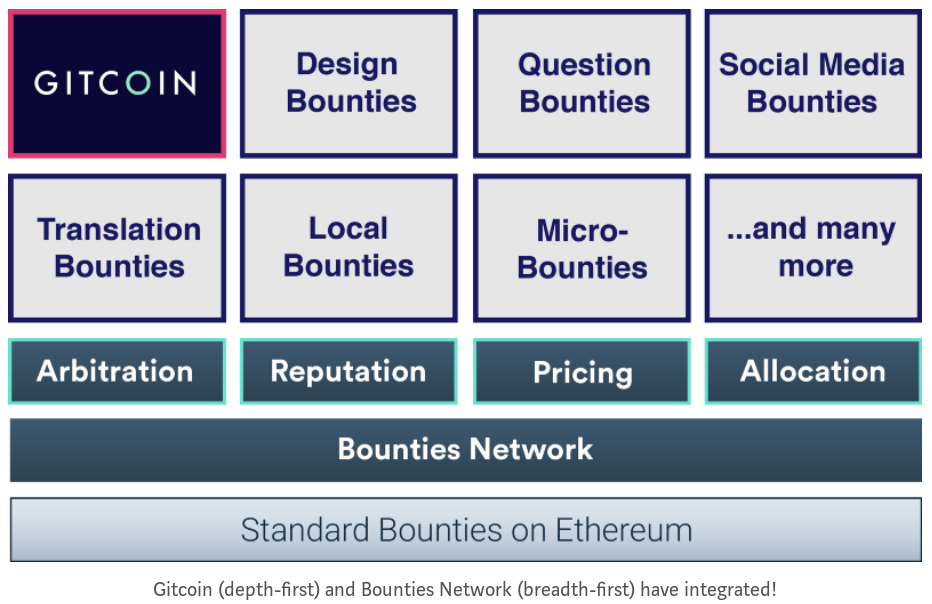
\includegraphics[width=10cm]{../pics/ConsenSys/bounties_network_stack}
		\caption{\tiny\url{https://medium.com/gitcoin/integrating-standard-bounties-dc4cf62bf814}}
	\end{figure}
	\tiny \copyright \href{https://www.consensys.net}{ConsenSys (2018)}
}


% 
% ======================================================================================================
%                                     ColliderX
% ======================================================================================================
\section{ColliderX: the world-first crowdfunded R\&D Hub focusing on Blockchain and related technologies}

% Going into more details in the next slides
%\frame{
%	\frametitle{\citeauthor{colliderx}} %ColliderX
%	\framesubtitle{\url{https://www.collider-x.org}}
%	\begin{itemize}
%		\item World-first Open Source Crowdfunded R\&D Hub focusing on Blockchain and related technologies (AI, IoT, ...)
%		\pause
%		\item Building \href{http://www3.weforum.org/docs/WEF_Realizing_Potential_Blockchain.pdf}{the digital infrastructure of tomorrow}
%		\pause
%		\item Now building a Blockchain \href{https://www.ic.gc.ca/eic/site/093.nsf/eng/00003.html}{Innovation Supercluster} in Canada
%		\pause
%		\item Open to all researchers/developers/tinkerers and backers in the world
%	\end{itemize}
%}

\frame{
	\frametitle{ColliderX}
	\begin{block}{Vision}
		ColliderX is a unique model for unbiased, ground-breaking R\&D that bridges the gap between industry problems and pure academic or corporate research.
		\hfill--\citeauthor{wef-tapscott2017} (\citeyear{wef-tapscott2017})
	\end{block}
	\begin{figure} % 
		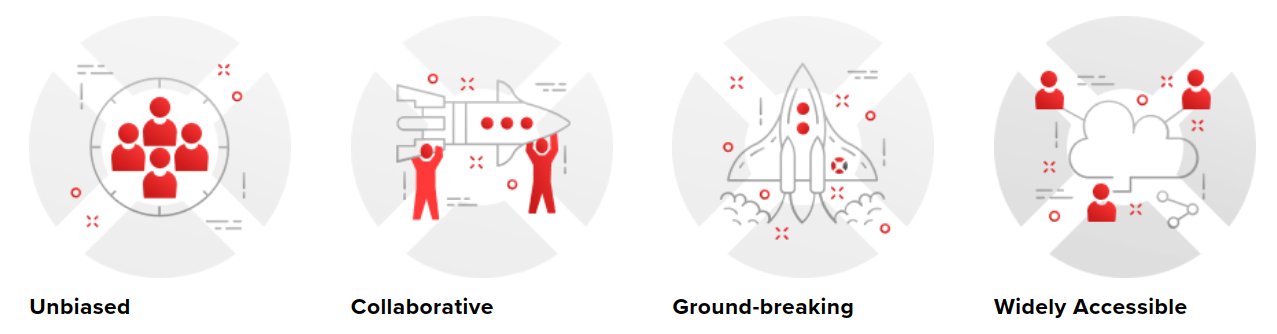
\includegraphics[width=10cm]{../pics/colliderx/research_attributes}
	\end{figure}
}

\frame{
	\frametitle{How to engage with ColliderX?}
	\begin{figure} % 
		
\includegraphics[width=10cm]{../pics/colliderx/tinkerers_backers}
	\end{figure}
}

\frame{
	\frametitle{Benefits for backers}
	\begin{figure} % 
		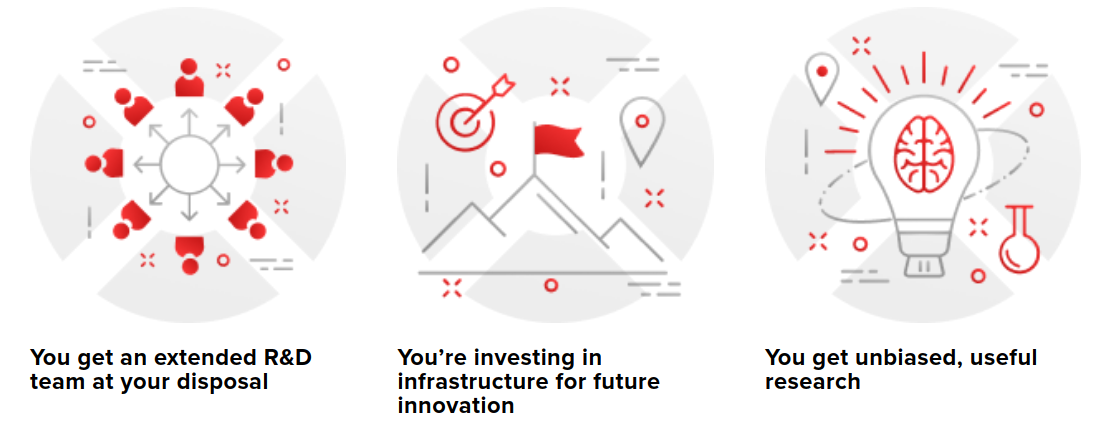
\includegraphics[width=10cm]{../pics/colliderx/backer_benefits}
	\end{figure}
}

\frame{
	\frametitle{ColliderX is global}
	\framesubtitle{and we're building a Blockchain Supercluster in Canada}
	\tikz[remember picture,overlay]
	  \node at
		([xshift=0cm,yshift=0cm]current page.center) 
		{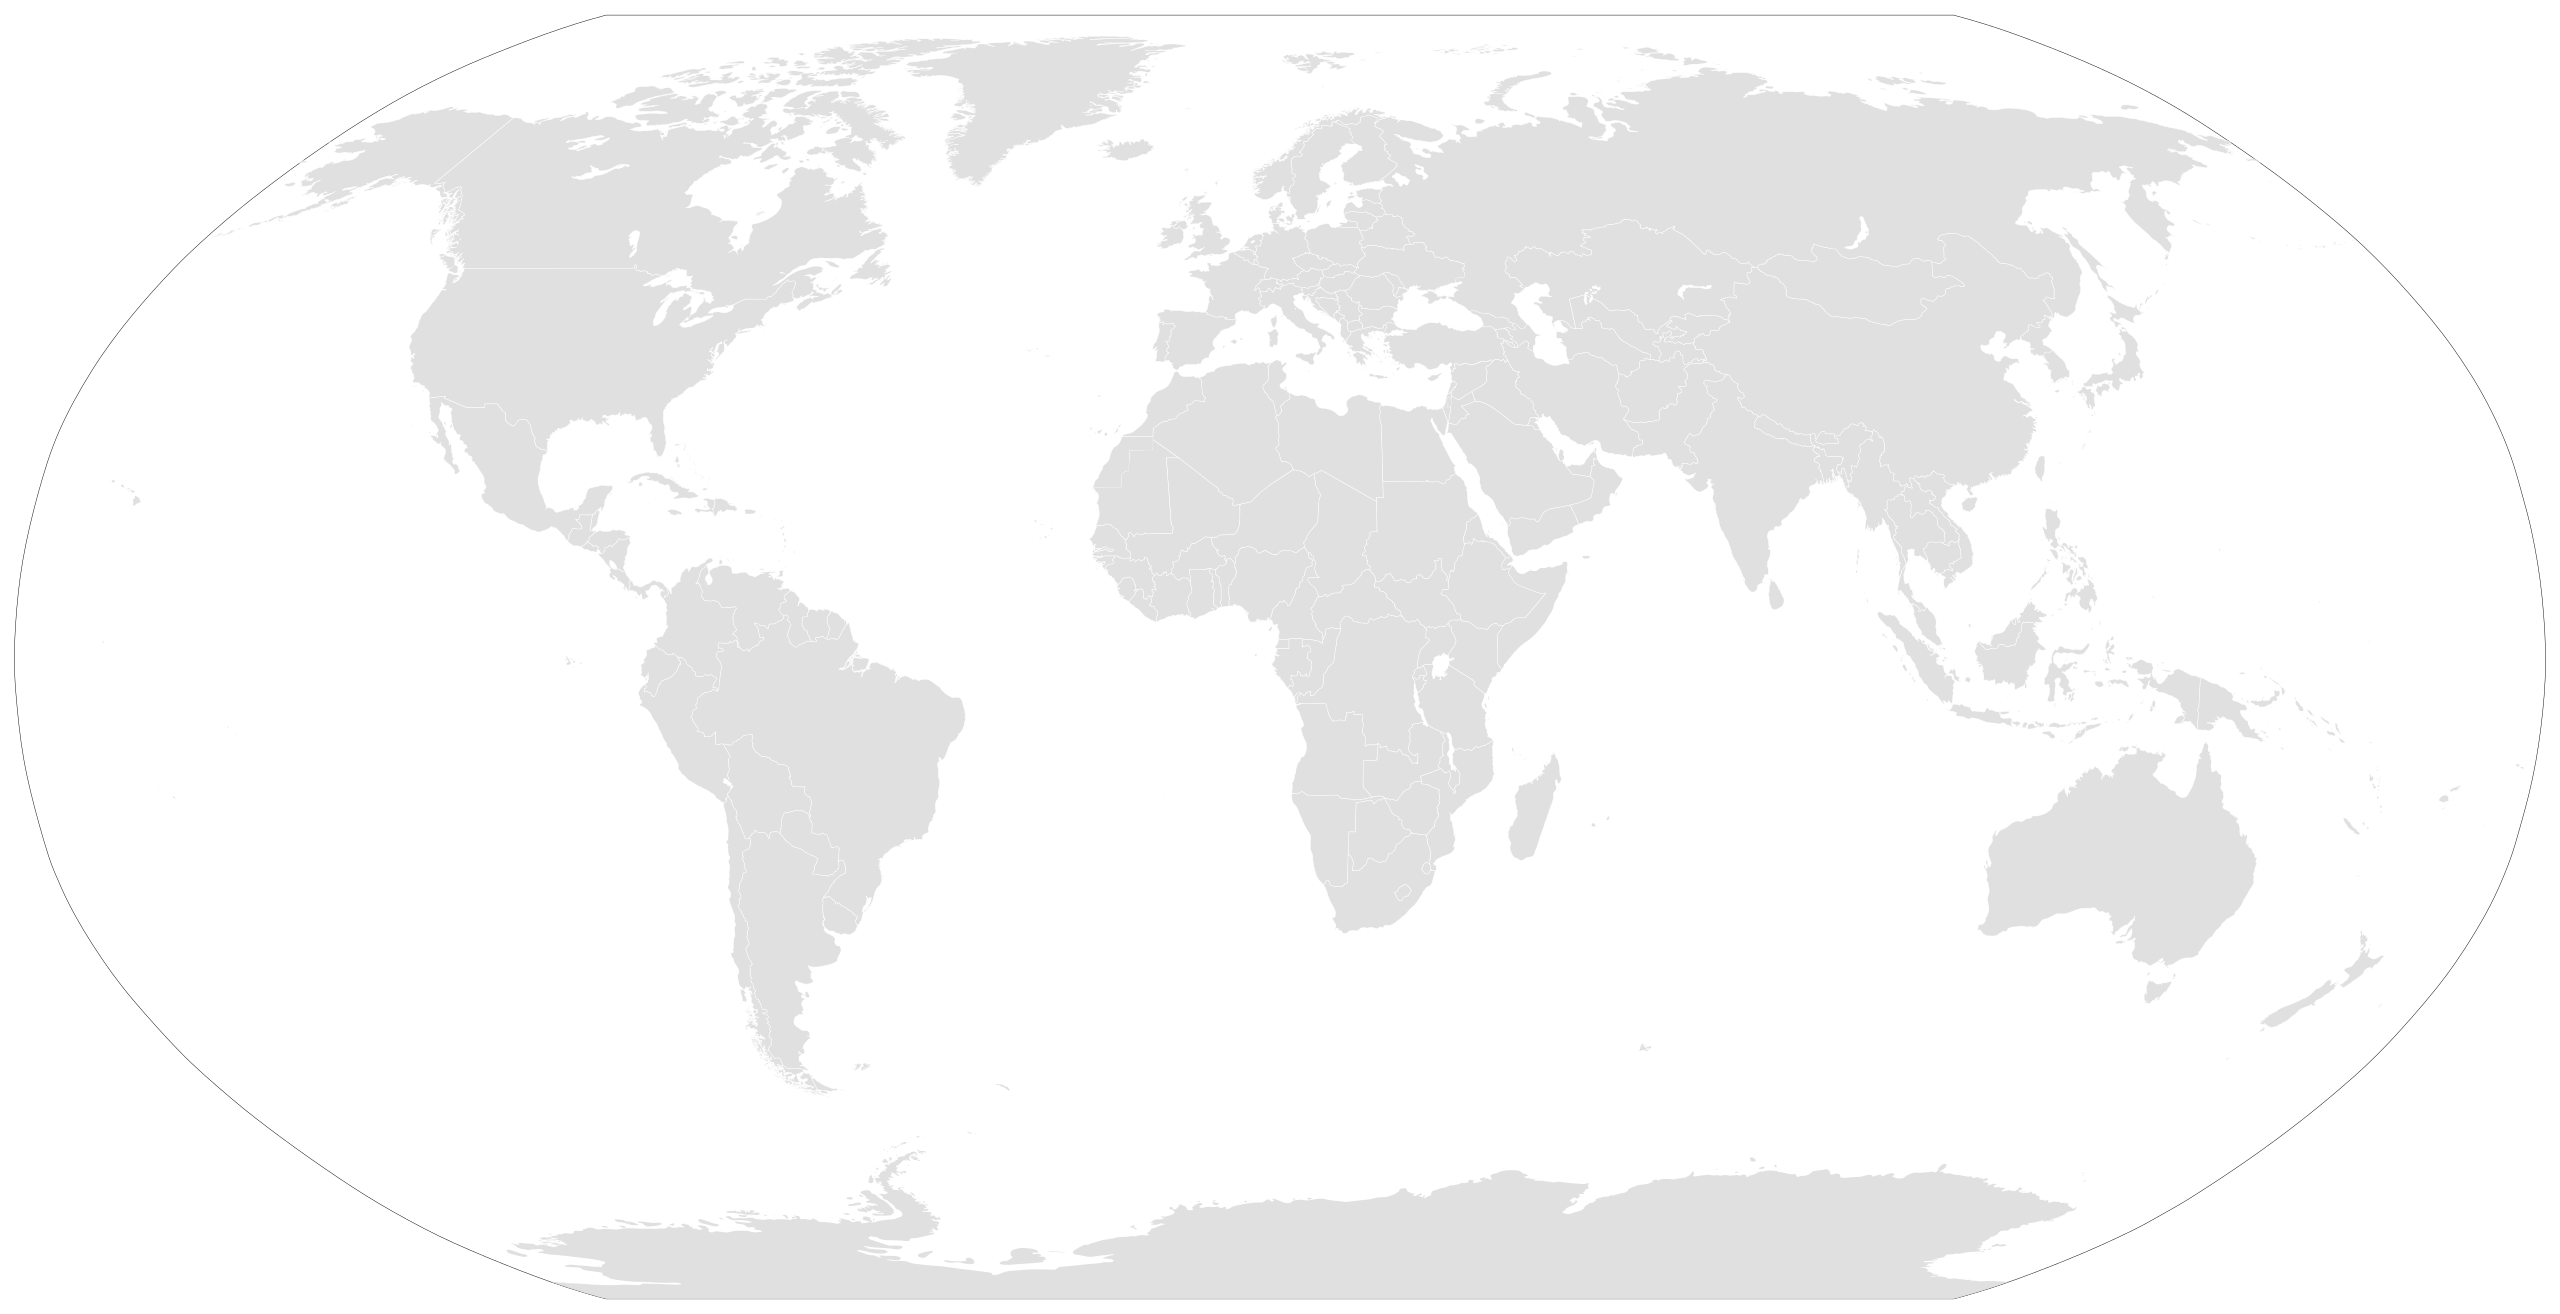
\includegraphics[width=11cm]{../pics/2560px-BlankMap-World6}};
	\tikz[remember picture,overlay]
	  \node at
		([xshift=3cm,yshift=2cm]current page.west)
		%([xshift=10.5cm,yshift=-3cm]current page.west)
		{
\includegraphics[height=.8cm]{../pics/colliderx/fabulousfive_dirty_transparent}};
	%\begin{figure} % 
	%	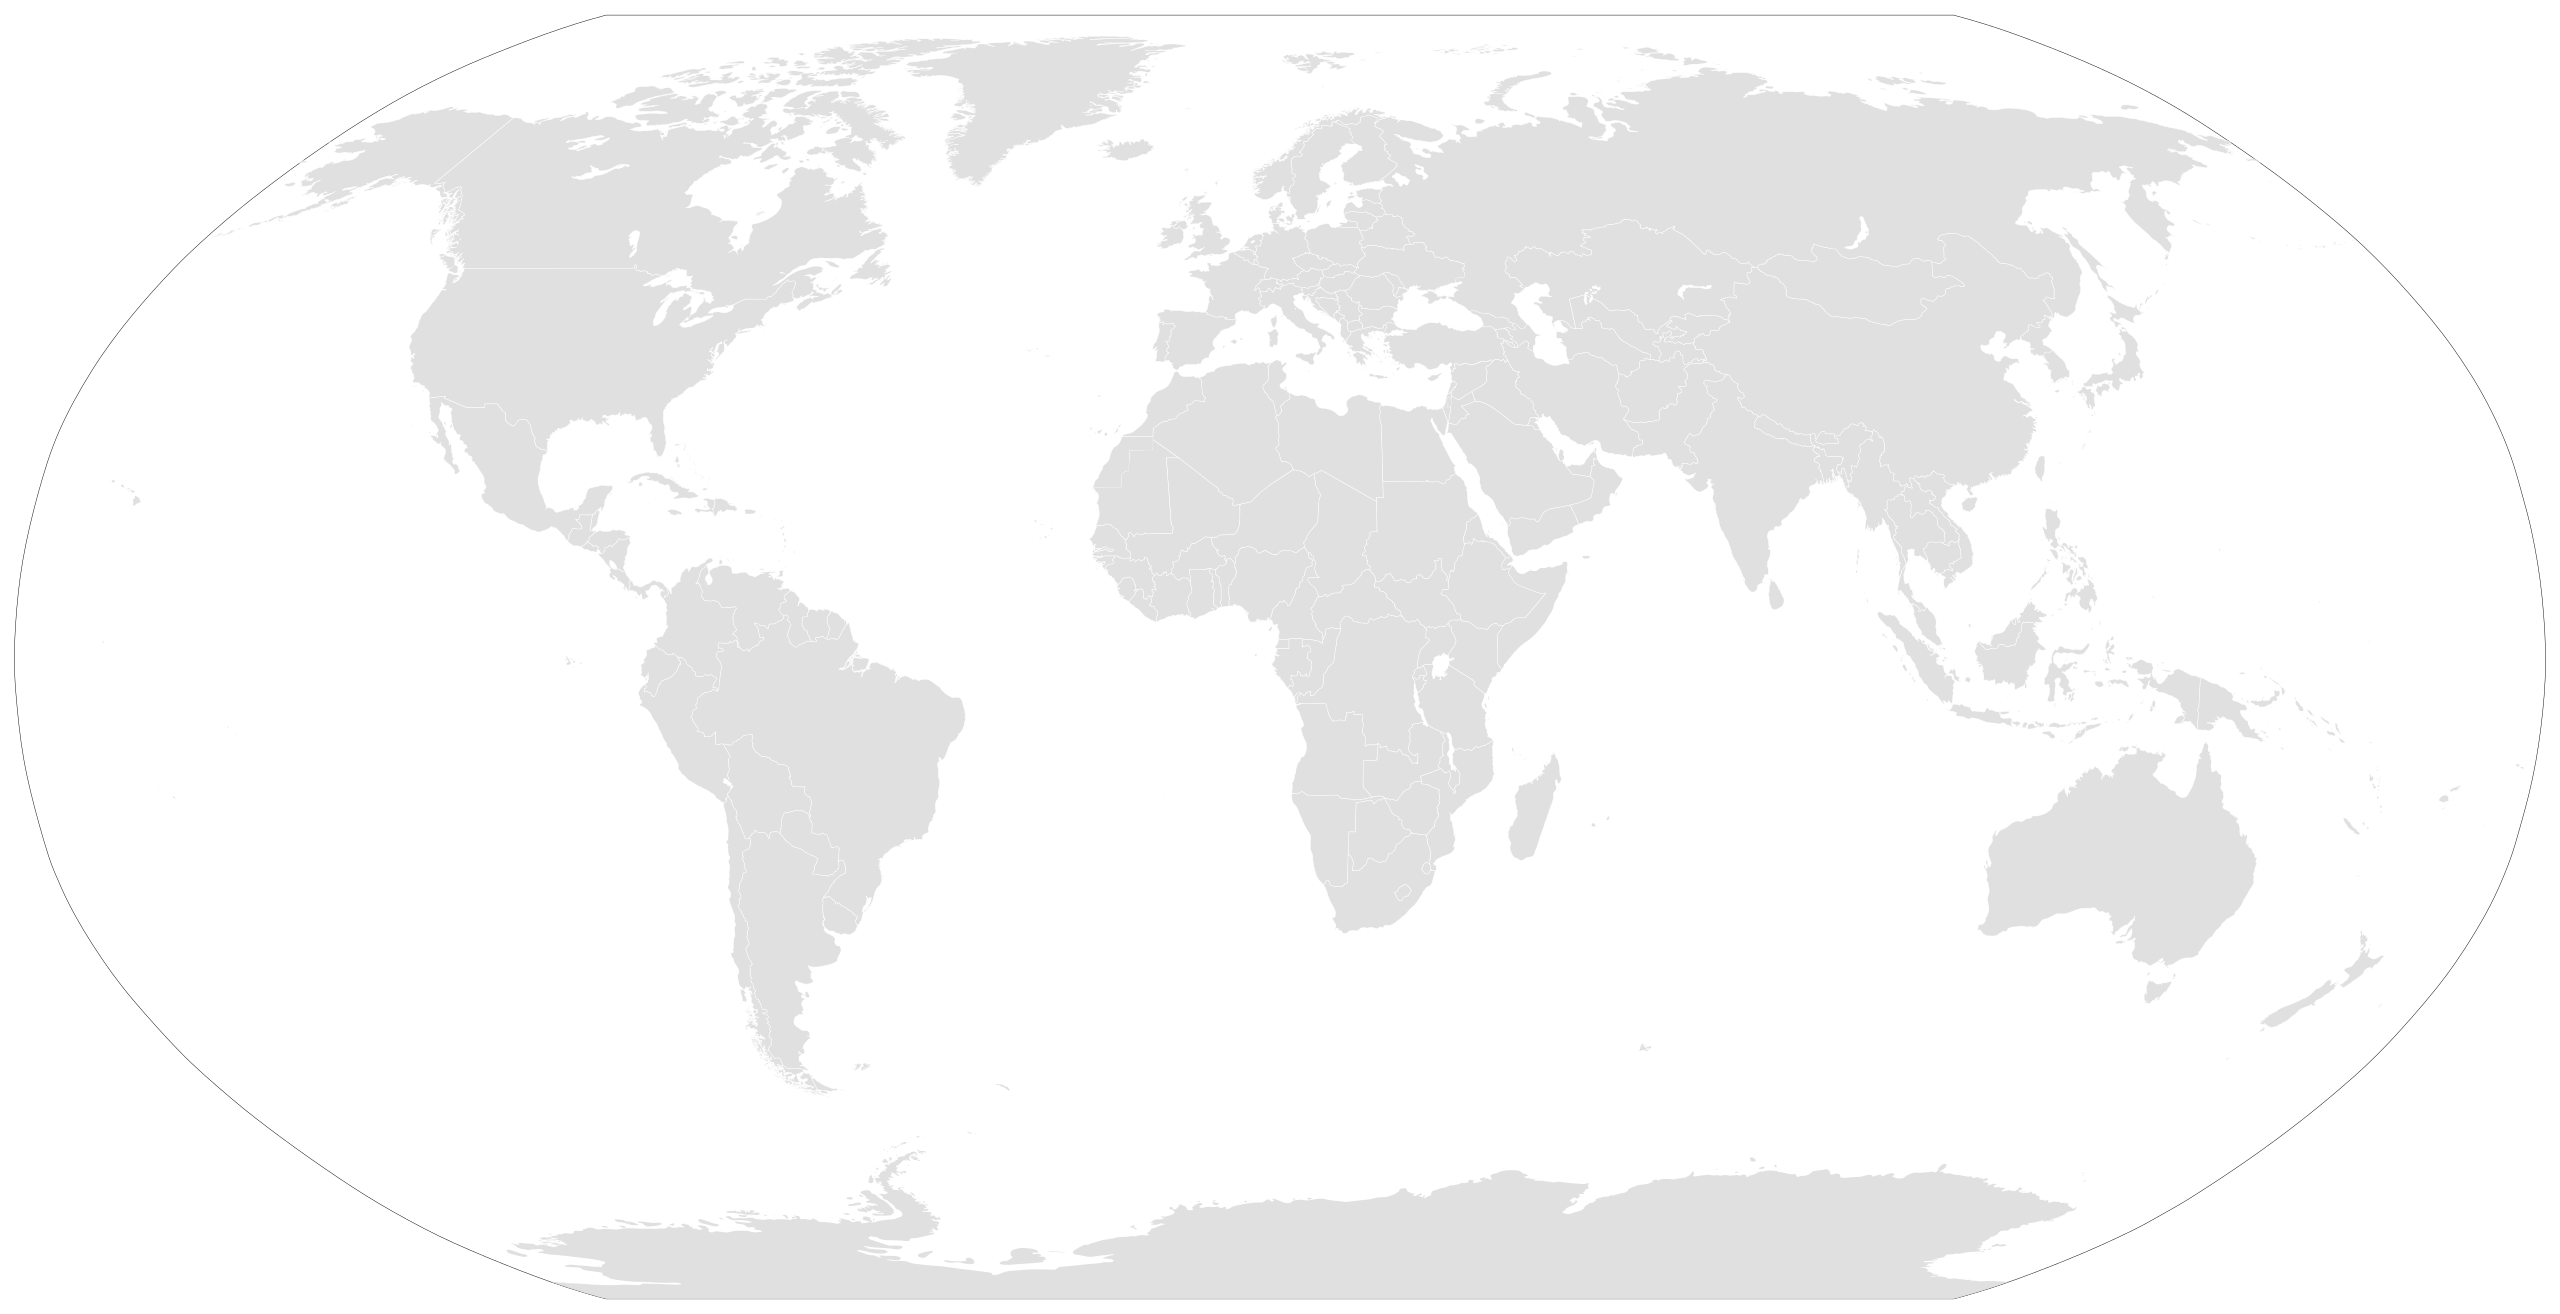
\includegraphics[width=10cm]{../pics/2560px-BlankMap-World6}
	%\end{figure}
}

\frame{
	\frametitle{Call to Action}
	\centering
	\Huge
	Submit your project proposal today at \url{www.collider-x.org}!
}

